\documentclass[12pt]{article}

\usepackage{amsmath}
\usepackage{amssymb}
\usepackage{amsthm}
\usepackage[pdftex]{graphicx}
\usepackage{setspace}
\usepackage{caption}
\usepackage{subcaption}
\usepackage{float}
\usepackage[margin=1in]{geometry}
\usepackage{listings}
\usepackage{textcomp}
\usepackage{multicol}
\usepackage[toc,page]{appendix}
\usepackage{listings}
\usepackage{fancyvrb}
\usepackage{hyperref}
\usepackage{lstbayes}
\usepackage{booktabs}

\usepackage[usenames,dvipsnames]{color}
\definecolor{DGrey}{gray}{0.25}
\definecolor{MGrey}{gray}{0.50}
\definecolor{LGrey}{gray}{0.75}

\usepackage[ruled,vlined,linesnumbered]{algorithm2e}
\newcommand\mycommfont[1]{\footnotesize\ttfamily\textcolor{Gray}{#1}}
\SetCommentSty{mycommfont}

\usepackage{inconsolata}

\usepackage[parfill]{parskip}
\setlength{\parindent}{0pt}
\setlength{\parskip}{\baselineskip}

\newcommand{\et}{e^{i\theta}}
\newcommand{\oo}{\mathcal{O}}
\newcommand{\skipline}{\bigskip\bigskip\bigskip}

\lstdefinestyle{Rsty} { 
    language=R,                         % the language of the code
    basicstyle=\footnotesize\ttfamily,  % the size of the fonts that are used for the code
    numbers=left,                       % where to put the line-numbers
    numberstyle=\footnotesize\color{LGrey},      % the style that is used for the line-numbers
    stepnumber=1,                       % the step between two line-numbers. If it is 1, each line
                                        % will be numbered
    numbersep=5pt,                      % how far the line-numbers are from the code
    backgroundcolor=\color{white},      % choose the background color. You must add \usepackage{color}
    showspaces=false,                   % show spaces adding particular underscores
    showstringspaces=false,             % underline spaces within strings
    showtabs=false,                     % show tabs within strings adding particular underscores
    frame=single,                       % adds a frame around the code
    rulecolor=\color{black},            % if not set, the frame-color may be changed on line-breaks within not-black text (e.g. commens (green here))
    tabsize=2,                          % sets default tabsize to 2 spaces
    captionpos=b,                       % sets the caption-position to bottom
    breaklines=true,                    % sets automatic line breaking
    breakatwhitespace=false,            % sets if automatic breaks should only happen at whitespace
    keywordstyle=\color{DGrey},     % keyword style
    commentstyle=\color{LGrey},   % comment style
    stringstyle=\color{MGrey},    % string literal style
    literate={<-}{{$\gets$}}1,           % prettier assignment arrows
    xleftmargin=4.0ex,
    deletekeywords={I,density,rect,_,palette,data,scale,panel,R,frame,labels,options}
}

\lstnewenvironment{R}
{\lstset{style=Rsty}}
{}

\lstdefinestyle{Stansty} { 
    language=Stan,                         % the language of the code
    basicstyle=\footnotesize\ttfamily,  % the size of the fonts that are used for the code
    numbers=left,                       % where to put the line-numbers
    numberstyle=\footnotesize\color{LGrey},      % the style that is used for the line-numbers
    stepnumber=1,                       % the step between two line-numbers. If it is 1, each line
                                        % will be numbered
    numbersep=5pt,                      % how far the line-numbers are from the code
    backgroundcolor=\color{white},      % choose the background color. You must add \usepackage{color}
    showspaces=false,                   % show spaces adding particular underscores
    showstringspaces=false,             % underline spaces within strings
    showtabs=false,                     % show tabs within strings adding particular underscores
    frame=single,                       % adds a frame around the code
    rulecolor=\color{black},            % if not set, the frame-color may be changed on line-breaks within not-black text (e.g. commens (green here))
    tabsize=2,                          % sets default tabsize to 2 spaces
    captionpos=b,                       % sets the caption-position to bottom
    breaklines=true,                    % sets automatic line breaking
    breakatwhitespace=false,            % sets if automatic breaks should only happen at whitespace
    keywordstyle=\color{DGrey},     % keyword style
    commentstyle=\color{LGrey},   % comment style
    stringstyle=\color{MGrey},    % string literal style
    %literate={<-}{{$\gets$}}1,           % prettier assignment arrows
    xleftmargin=4.0ex,
    deletekeywords={T}
}

\lstnewenvironment{Stan}
{\lstset{style=Stansty}}
{}

\renewcommand{\arraystretch}{2}

\begin{document}

\noindent
{\LARGE {\bf Parameter Fitting} }
\\\\
Dexter Barrows\\
\today

\section{Fitting Setup}

	Now that we have established which methods we wish to evaluate the efficacy of for epidemic forecasting, it is prudent to see how they perform when fitting parameters for a known epidemic model. We have already seen how they perform when fitting parameters for a model with a deterministic evolution process and observation noise, but a more realistic model will have both process and observation noise.

	To form such a model, we will take a deterministic SIR ODE model given by

	\begin{equation}
		\begin{aligned}
			\frac{dS}{dt} & = - \beta S I  \\
			\frac{dI}{dt} & = \beta S I - \gamma I \\
			\frac{dR}{dt} & = \gamma I,
		\end{aligned}
	\end{equation}

	and add process noise by allowing $\beta$ to embark on a geometric random walk given by

	\begin{equation}\label{betaautoreg}
		\beta_{t+1} = \exp \left( \log(\beta_{t}) + \eta (\log(\bar{\beta}) - \log(\beta_{t})) + \epsilon_{t} \right).
	\end{equation}

	We will take $\epsilon_{t}$ to be normally distributed with standard deviation $\rho^2$ such that $\epsilon_{t} \sim \mathcal{N}(0,\rho^2)$. The geometric attraction term constrains the random walk, the force of which is $\eta \in [0,1]$. If we take $\eta = 0$ then the walk will be unconstrained; if we let $\eta = 1$ then all values of $\beta_t$ will be independent from the previous value (and consequently all other values in the sequence).

	When $\eta \in (0,1)$, we have an autoregressive process of order 1 on the logarithmic scale of the form

	\begin{equation}
		X_{t+1} = c + \rho X_t + \epsilon_t ,
	\end{equation}

	where $\epsilon_t$ is normally distributed noise with mean 0 and standard deviation $\sigma_E$. This process has a theoretical expected mean of $\mu = c / (1 - \rho)$ and variance $\sigma = \sigma_E^2 / (1 - \rho^2)$. If we choose $\eta = 0.5$, the resulting log-normal distribution has a mean of $6.80 \times 10^{-4}$ and standard deviation of $4.46 \times 10^{-4}$.

	Simulating the process in Equation [\ref{betaautoreg}] with $\eta = 0.5$ gives us the plot in Figure [\ref{betaplot}] below.

	\begin{figure}[H]
        \centering
        \captionsetup{width=.8\linewidth}
        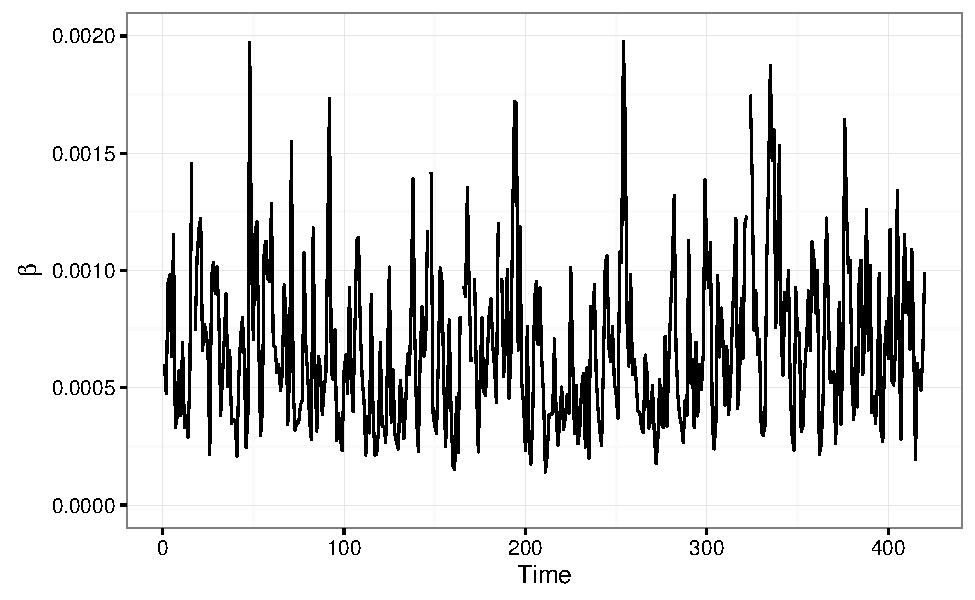
\includegraphics[width=0.8\textwidth]{./images/betaplot.pdf}
        \caption{Simulated geometric autoregressive process show in Equation [\ref{betaautoreg}].}
        \label{betaplot}
    \end{figure}

    We can obtain the corresponding density plot of the values in Figure [\ref{betaplot}], shown in Figure [\ref{betadensity}].

    \begin{figure}[H]
        \centering
        \captionsetup{width=.8\linewidth}
        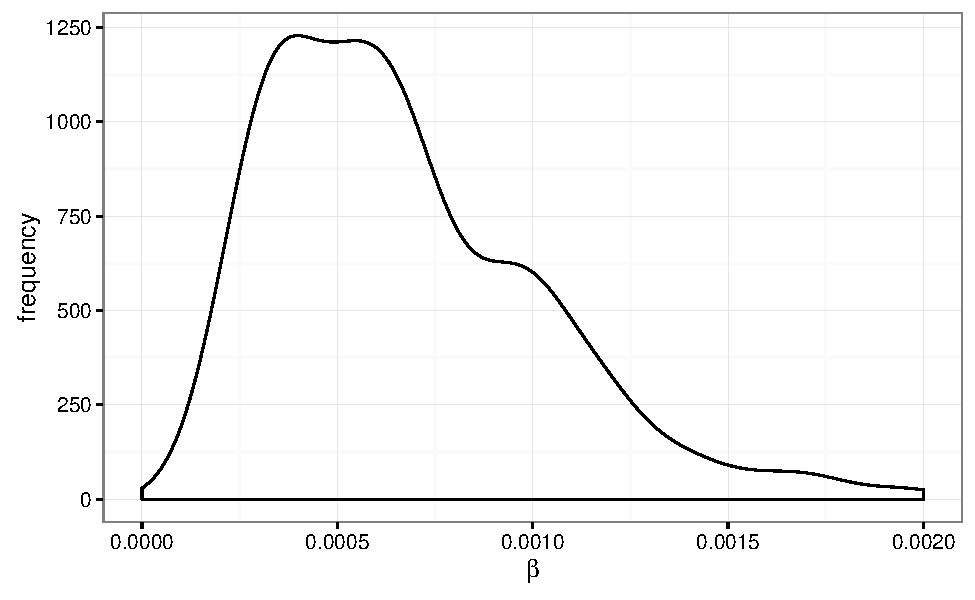
\includegraphics[width=0.8\textwidth]{./images/betadensity.pdf}
        \caption{Density plot of values shown if Figure[\ref{betaplot}].}
        \label{betadensity}
    \end{figure}

    We see a density plot similar in shape to the desired density, and the geometric random walk displays dependence on previous values. Further the mean of this distribution was calculated to be $6.92 \times 10^{-4}$ and standard the deviation to be $3.99 \times 10^{-4}$, which are very close to the theoretical values.

    If we take the full stochastic SIR system and evolve it using an Euler stepping scheme with a step size of $h = 1/7$, for 1 step per day, we obtain the plot in Figure [\ref{sirmean}].

    \begin{figure}[H]
        \centering
        \captionsetup{width=.8\linewidth}
        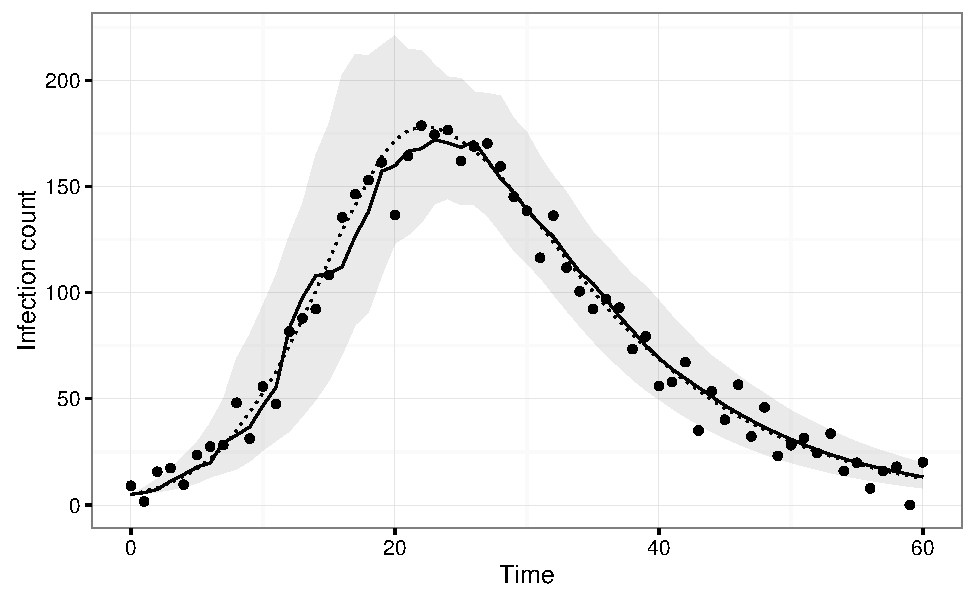
\includegraphics[width=0.8\textwidth]{./images/sirmean.pdf}
        \caption{Stochastic SIR model simulated using an explicit Euler stepping scheme. The solid line is a single random trajectory, the dots show the data points obtained by adding in observation error defined as $\epsilon_{obvs} = \mathcal{N}(0,10)$, and the grey ribbon is centre 95th quantile from 100 random trajectories.}
        \label{sirmean}
    \end{figure}

\section{Calibrating Samples}

	In order to compare HMCMC and IF2 we need to set up a fair and theoretically justified way to select the number of samples to draw for the HMCMC iterations and the number of particles to use for IF2. We assume that we are working with a problem that has an unknown real solution, so we use the Monte Carlo Standard Error (MCSE).

	Suppose we are using a Monte-Carlo based method to obtain an estimate $\hat{\mu}_{n}$ for a quantity $\mu$, where $n$ is the number of samples. Then the Law of Large Numbers says that $\hat{\mu}_{n} \rightarrow \mu$ as $n \rightarrow \infty$. Further, the Central Limit Theorem says that the error $\hat{\mu}_{n} - \mu$ should shrink with number of samples such that $\sqrt{n} (\hat{\mu}_{n} - \mu) \rightarrow \mathcal{N}(0,\sigma^2)$ as $n \rightarrow \infty$, where $\sigma^2$ is the variance of the samples drawn.

	We of course do not know $\mu$, but the above allows us to obtain an estimate $\hat{\sigma}_n$ for $\sigma$ given a number of samples $n$ as

	\begin{equation}
		\hat{\sigma}_n = \sqrt{\frac{1}{n} \sum_{i=1}^{n} (X_i - \hat{\mu}) },
	\end{equation}

	which is known as the Monte Carlo Standard Error.

	We can modify this formula to account for multiple variables by replacing the single variance measure sum by

	\begin{equation}
		\Theta^* V (\Theta^*)^T
	\end{equation}

	where $\Theta^*$ is a row vector containing the reciprocals of the means of the parameters of interest, and $V$ is the variance-covariance matrix with respect to the same parameters. This in effect scales the variances with respect to their magnitudes and accounts for covariation between parameters in one fell swoop. We also divide by the number of parameters, yielding

	\begin{equation}
		\hat{\sigma}_n = \sqrt{\frac{1}{n} \frac{1}{P} \Theta^* V (\Theta^*)^T }
	\end{equation}

	where $P$ is the number of particles.

	The goal here is to then pick the number of HMCMC samples and IF2 particles to yield similar MCSE values. To do this we picked a combination of parameters for RStan that yielded decent results when applied to the stochastic SIR model specified above, calculated the resulting mean MCSE across several model fits, and isolated the expected number of IF2 particles needed to obtain the same value. This was used as a starting value to ``titrate'' the IF2 iterations to the same point.

	The resulting values were 1000 HMCMC warm-up iterations with 1000 samples drawn post-warm-up, and 2500 IF2 particles sent through 50 passes, each method giving an approximate MCSE of 0.0065.

\section{IF2 Fitting}

	Now we will use an implementation of the IF2 algorithm to attempt to fit the stochastic SIR model to the previous data. The goal here is just parameter inference, but since IF2 works by applying a series on particle filters we essentially get the average system state estimates for a very small additional computational cost. Hence, we will will also look at that estimated behaviour in addition the the parameter estimates.

	The code used here is a mix of R and C++ implemented using RCpp. The fitting was undertaken using $2500$ particles with 50 IF2 passes and a cooling schedule given by a reduction in particle spread determined by $0.975^{p}$, where p is the pass number starting with 0.

	The MLE parameter estimates, taken to be the mean of the particle swarm values after the final pass, are shown in the table in Figure [\ref{fiterror}], along with the true values and the relative error.

	\begin{figure}[H]
		\centering
		{\small
		\begin{tabular}{cccccc}
			& & \multicolumn{2}{c}{IF2} & \multicolumn{2}{c}{HMCMC} \\
			\cmidrule[1.0pt](r){3-4} \cmidrule[1.0pt](r){5-6}
			Name & True	& Fit & Error & Fit & Error \\
			\cmidrule[1.0pt](r){1-1} \cmidrule[1.0pt](r){2-2} \cmidrule[1.0pt](r){3-3} \cmidrule[1.0pt](r){4-4} \cmidrule[1.0pt](r){5-5} \cmidrule[1.0pt](r){6-6}
			$R_0$ 				& 3.0 				 & 3.27 					& $9.08 \times 10^{-2}$ 	& $3.12$ 				& $1.05 \times 10^{-1}$		\\
			$r$ 				& $10^{-1}$  		 & $1.04 \times 10^{-1}$ 	& $3.61 \times 10^{-2}$ 	& $9.99 \times 10^{-2}$ & $-7.56 \times 10^{-4}$	\\
			Initial Infected 	& 5  				 & 7.90 					& $5.80 \times 10^{-1}$ 	& $6.64$ 				& $3.28 \times 10^{-1}$ 	\\
			$\sigma$ 			& 10   				 & 8.84 					& $-1.15 \times 10^{-1}$ 	& $8.5$ 				& $-1.50 \times 10^{-1}$	\\
			$\eta$ 				& $5 \times 10^{-1}$ & $5.87 \times 10^{-1}$ 	& $1.73 \times 10^{-1}$ 	& $4.57 \times 10^{-1}$ & $-8.27 \times 10^{-2}$ 	\\
			$\varepsilon_{err}$ & $5 \times 10^{-1}$ & $1.63 \times 10^{-1}$ 	& $-6.73 \times 10^{-1}$ 	& $1.60 \times10^{-1}$  & $-6.80 \times 10^{-1}$
		\end{tabular}}
	    \caption{Fitting errors.}
        \label{fiterror}
    \end{figure}


	From last IF2 particle filtering iteration, the mean state values from the particle swarm at each time step are shown with the true underlying state and data in the plot in Figure [\ref{if2state}].

	\begin{figure}[H]
        \centering
        \captionsetup{width=.8\linewidth}
        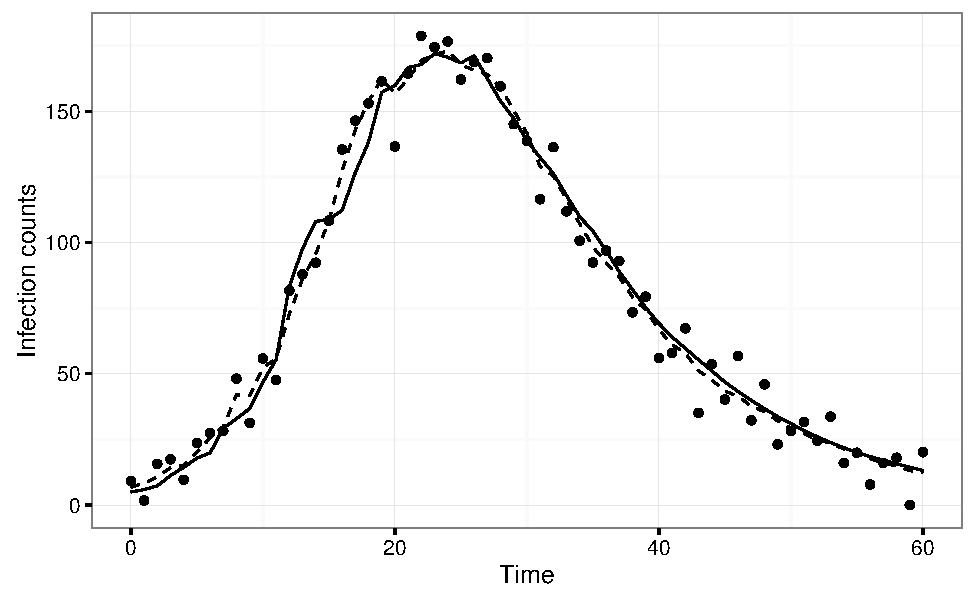
\includegraphics[width=0.8\textwidth]{./images/if2state.pdf}
        \caption{True system trajectory (solid line), observed data (dots), and IF2 estimated real state (dashed line).}
        \label{if2state}
    \end{figure}

\section{IF2 Convergence}

	Since IF2 is an iterative algorithm where each pass through he data is expected to push the parameter estimates towards the MLE, we can see the evolution of these estimates as a function of the pass number. Plots showing evolution of the mean estimates are shown if Figure [\ref{if2convergence}] for the six most critical parameters.

	\begin{figure}[H]
        \centering
        \captionsetup{width=.8\linewidth}
        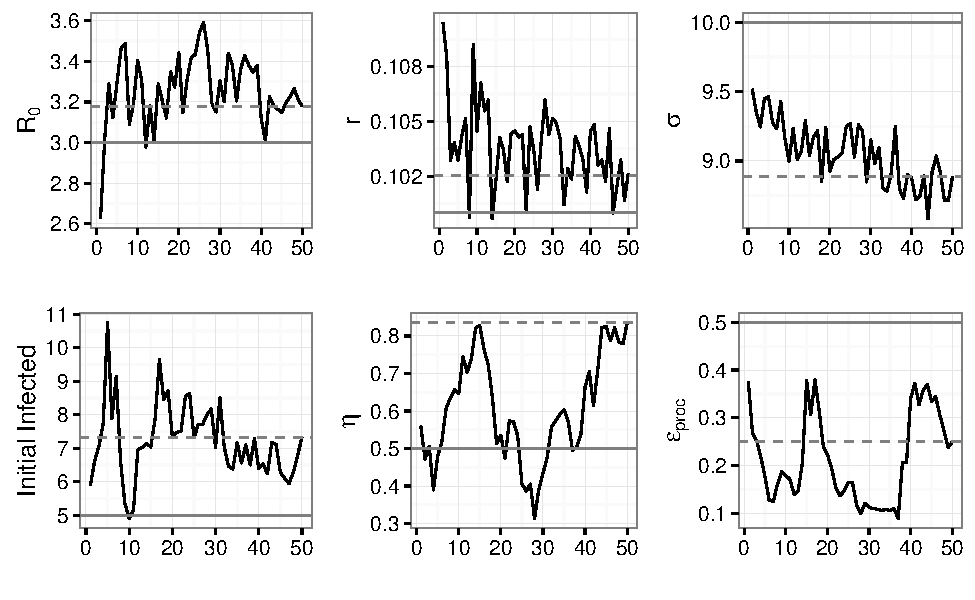
\includegraphics[width=0.8\textwidth]{./images/if2convergence.pdf}
        \caption{The horizontal axis shows the IF2 pass number. The solid black lines show the evolution of the ML estimates, the solid grey lines show the true value, and the dashed grey lines show the mean parameter estimates from the particle swarm after the final pass.}
        \label{if2convergence}
    \end{figure}

    Similarly, we can look at the evolution of the standard deviations of the parameter estimates from the particle swarm as a function of the pass number, shown in Figure [\ref{if2sdconvergence}] below.

    \begin{figure}[H]
        \centering
        \captionsetup{width=.8\linewidth}
        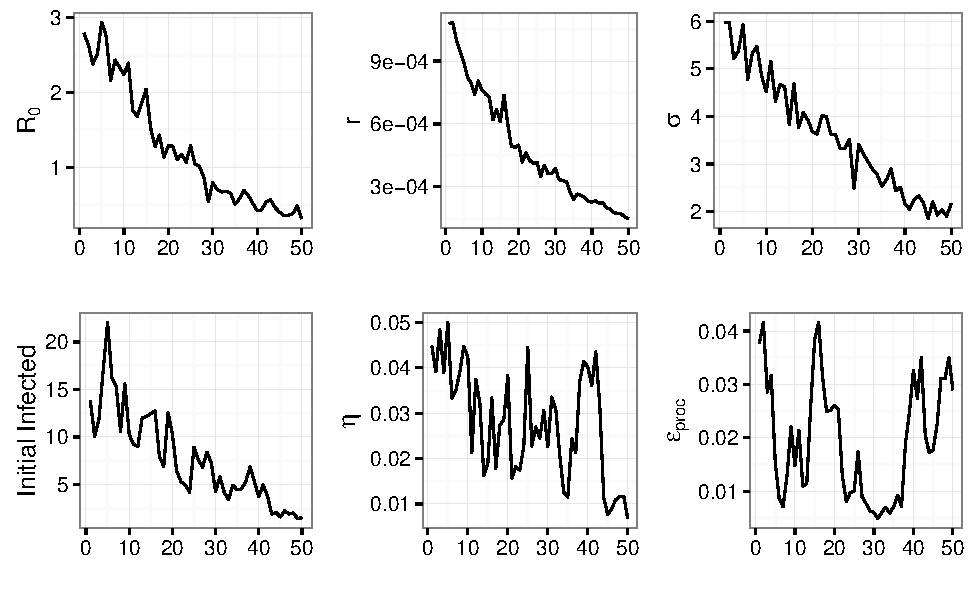
\includegraphics[width=0.8\textwidth]{./images/if2sdconvergence.pdf}
        \caption{The horizontal axis shows the IF2 pass number and the solid black lines show the evolution of the standard deviations of the particle swarm values.}
        \label{if2sdconvergence}
    \end{figure}

    As expected there is a downward trend in all plots, with a very strong trend in all but two of them.


\section{IF2 Densities}

	Of diagnostic importance are the densities of the parameter estimates given by the final parameter swarm. These are shown below if Figure [].

	\begin{figure}[H]
        \centering
        \captionsetup{width=.8\linewidth}
        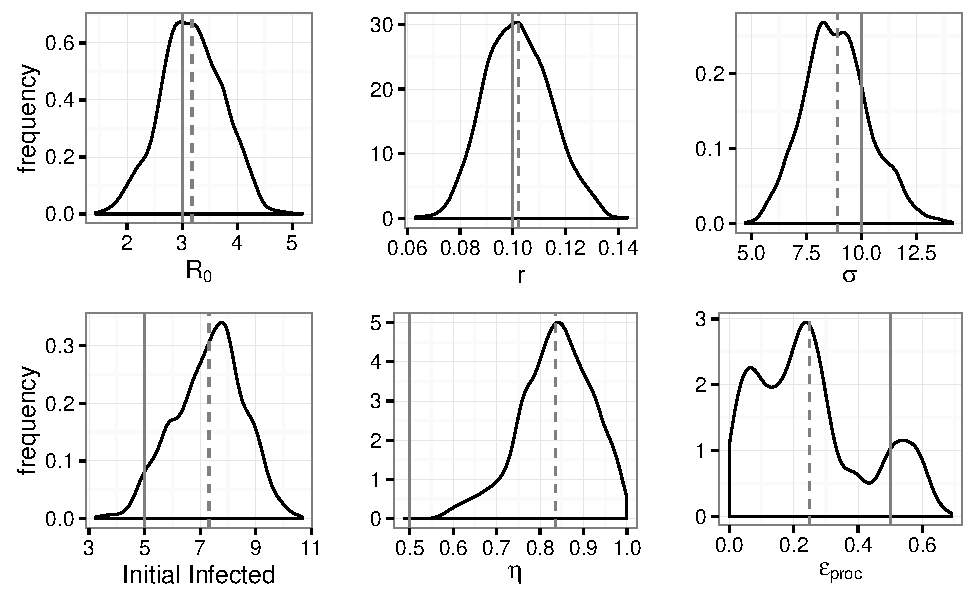
\includegraphics[width=0.8\textwidth]{./images/if2kernels.pdf}
        \caption{As before, the solid grey lines show the true parameter values and the dashed grey lines show the density means.}
        \label{if2kernels}
    \end{figure}

    It is worth noting that the IF2 parameters chosen were in part chosen so as to not artificially narrow these densities; a more aggressive cooling schedule and/or an increased number of passes would have resulted in much narrower densities, and indeed have the potential to collapse them to point estimates.

\section{HMCMC Fitting}

	We can use the Hamiltonian Monte Carlo algorithm implemented in the `Rstan` package to fit the stochastic SIR model as above. This was done with a single HMC chain of 2000 iterations with 1000 of those being warm-up iterations.

	The MLE parameter estimates, taken to be the means of the samples in the chain, were shown in the table in Figure [\ref{fiterror}] along with the true values and relative error.


\section{HMCMC Densities}

	The parameter estimation densities from the Stan HMCMC fitting are shown in Figure [\ref{hmckernels}] below.

	\begin{figure}[H]
        \centering
        \captionsetup{width=.8\linewidth}
        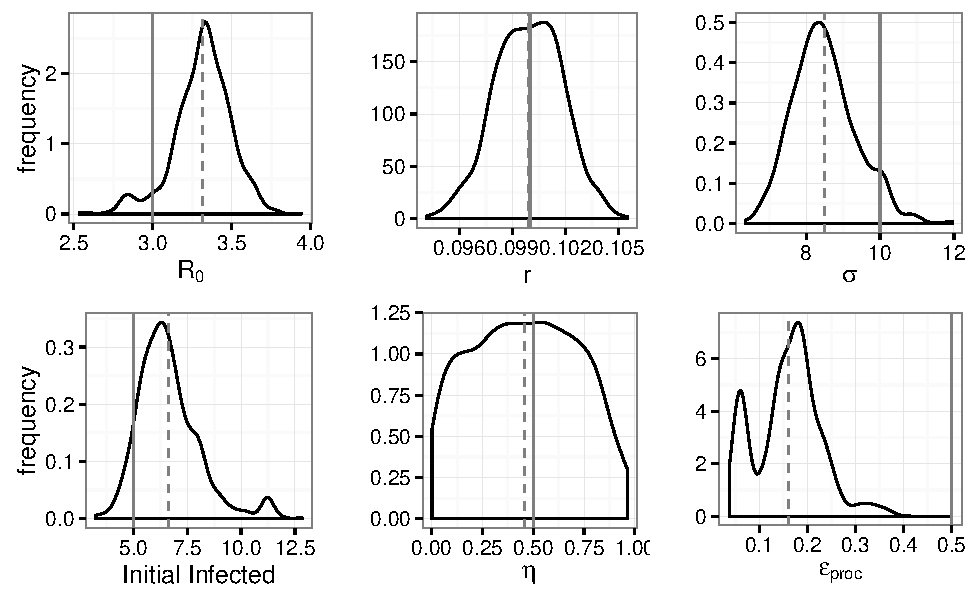
\includegraphics[width=0.8\textwidth]{./images/hmckernels.pdf}
        \caption{As before, the solid grey lines show the true parameter values and the dashed grey lines show the density means.}
        \label{hmckernels}
    \end{figure}

    the densities shown here represent a ``true'' MLE density estimate in that they represent HMC's attempt to directly sample from the parameter space according to the likelihood surface, unlike IF2 which is in theory only trying to get a ML point estimate. Hence, these densities are potentially more robust than those produced by the IF2 implementation.


\section{HMCMC and Bootstrapping}

	Unlike particle particle-filtering-based approaches, HMC does not produce state estimates as a by-product of parameter fitting, but we can use information about the stochastic nodes related to the noise in the $\beta$ geometric random walk to reconstruct state estimates. The results of 100 bootstrap trajectories is shown in Figure [\ref{hmcboot}].

	\begin{figure}[H]
        \centering
        \captionsetup{width=.8\linewidth}
        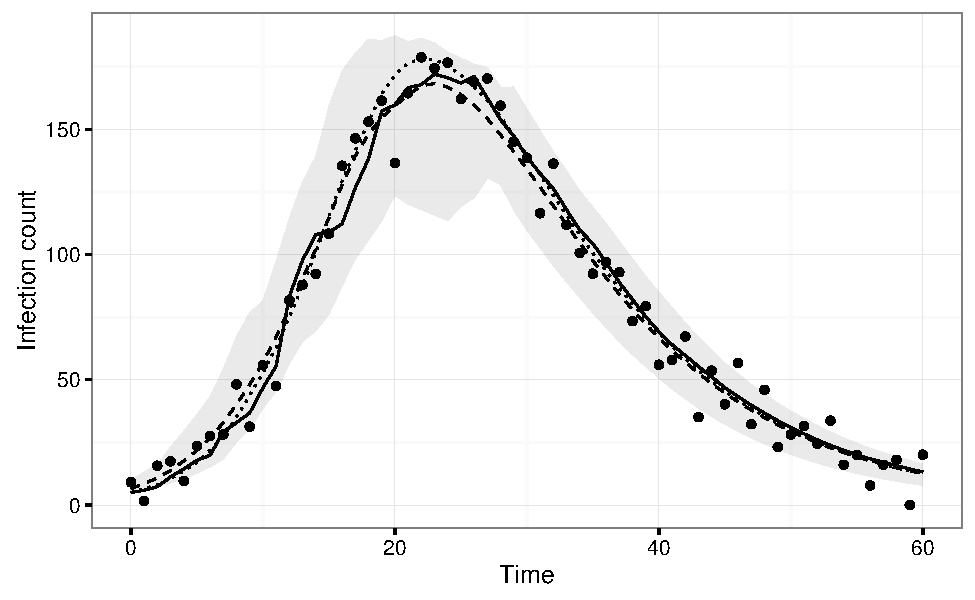
\includegraphics[width=0.8\textwidth]{./images/hmcboot.pdf}
        \caption{Result from 100 HMCMC bootstrap trajectories. The solid line shows the true states, the dots show the data, the dotted line shows the average system behaviour, the dashed line shows the bootstrap mean, and the grey ribbon shows the centre 95th quantile of the bootstrap trajectories.}
        \label{hmcboot}
    \end{figure}


\section{Multi-trajectory Parameter Estimation}

	Here we fit the stochastic SIR model to 200 random independent trajectories using each method and examine the density of the point estimates produced. 

    \begin{figure}[H]
        \centering
        \captionsetup{width=.8\linewidth}
        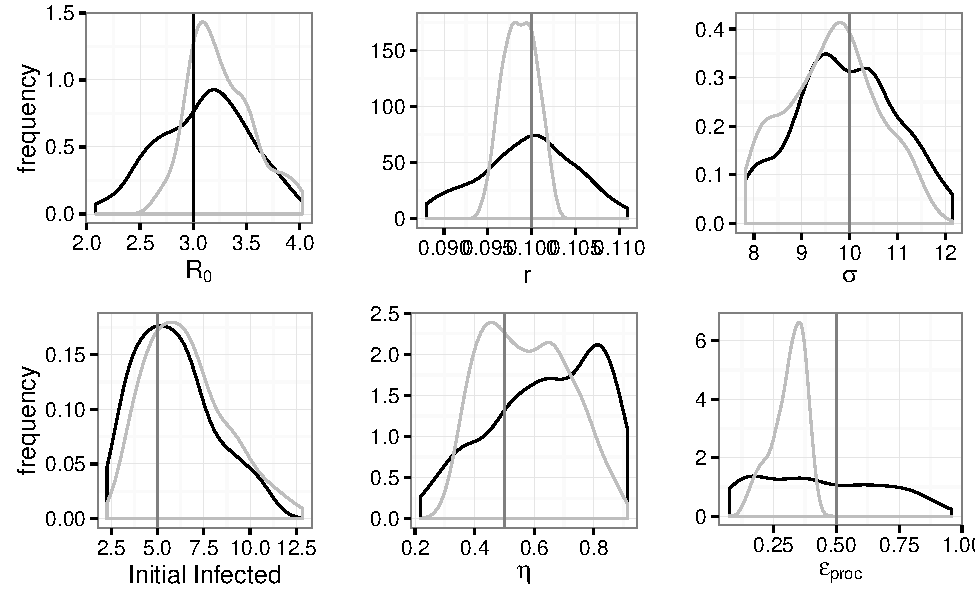
\includegraphics[width=0.8\textwidth]{./images/combined-multi.pdf}
        \caption{IF2 point estimate densities are shown in black and HMCMC point estimate densities are shown in grey. The vertical black lines show the true parameter values.}
        \label{combinedmulti}
    \end{figure}

    The densities by and large display similar coverage, with the IF2 densities for $r$ and $\varepsilon_{proc}$ showing slightly wider coverage than the HMCMC densities for the same parameters.

    The running times for each algorithm are summarized in Figure [\ref{timeplot}] below.

	\begin{figure}[H]
        \centering
        \captionsetup{width=.8\linewidth}
        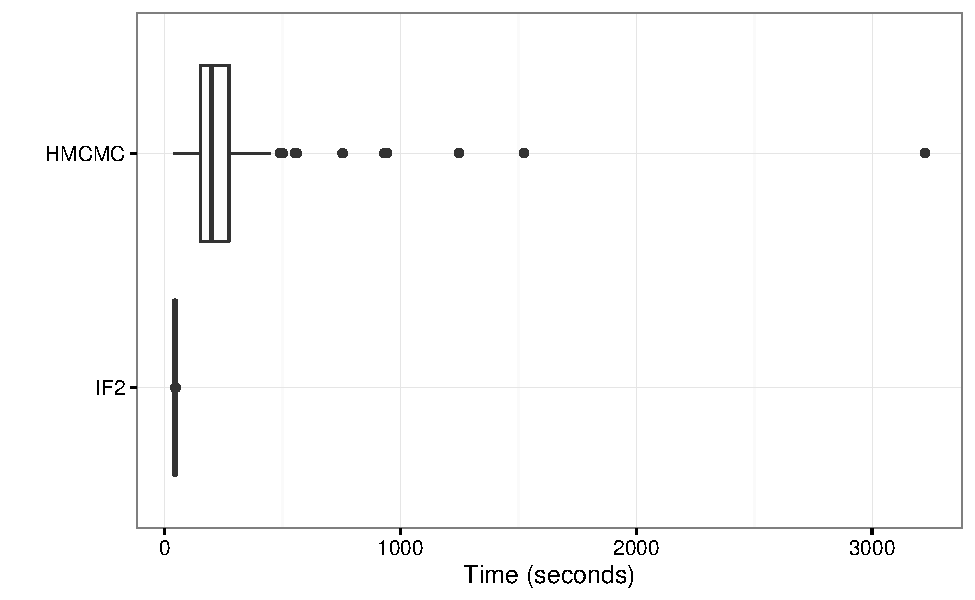
\includegraphics[width=0.8\textwidth]{./images/timeplot.pdf}
        \caption{Fitting times for IF2 and HMCMC, in seconds. The centre box in each plot shows the centre 50th quantile, with the bold centre line showing the median.}
        \label{timeplot}
    \end{figure}

    The average running times were approximately 45.5 seconds and 257.4 seconds for IF2 and HMCMC respectively, representing a 5.7x speedup for IF2 over HMCMC. While IF2 may be able to fit the model to data faster than HMCMC, we are obtaining less information; this will become important in the next section. Further, the results in Figure [\ref{timeplot}] show that while the running time for IF2 is relatively fixed, the times for HMCMC are anything but, showing a wide spread of potential times.



\end{document}